\chapter{Resultados, conclusiones y recomendaciones}

\section{Resultados}

\subsection{Implementación del EMD en Fortran}

\noindent La implementación del método EMD en Fortran se realizó siguiendo el planteamiento de la sección \ref{EMD}. En la figura \ref{fig:emd_comparison} se observa que nuestra implementación genera, en promedio, un mayor número de IMFs respecto de las implementaciones de Python (python 3) y Matlab (versión R2021a), para cualquiera de las series temporales.

\begin{figure}[H]
\centering
\subfigure{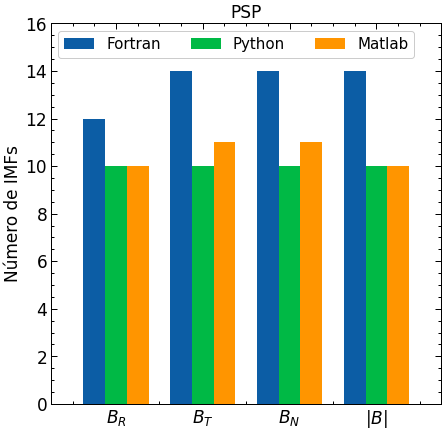
\includegraphics[scale=0.47]{Imagenes/number_imfs_PSP.png}\label{comparison1}}
\subfigure{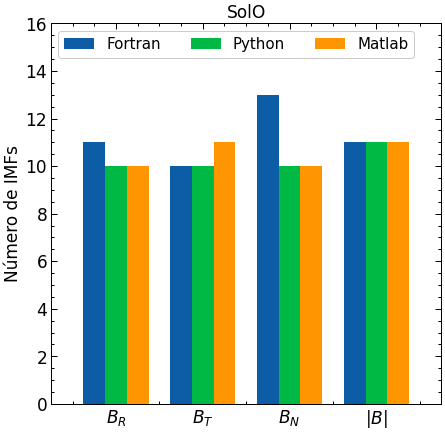
\includegraphics[scale=0.47]{Imagenes/number_imfs_SolO.png}\label{comparison2}}
\caption{Comparación en el número de IMFs resultantes de la descomposición de las series temporales del campo magnético mediante el método EMD en Fortran, Python y Matlab. Izquierda: PSP; derecha: SolO.}
\label{fig:emd_comparison}
\end{figure}

Los resultados dependen de la implementación exacta del método, lo que explica la variabilidad en el número de IMFs entre las diferentes implementaciones. Las principales diferencias pueden deberse al tipo de interpolación para el cálculo de las envolventes, las condiciones de frontera de las envolventes y los criterios de detenimiento del proceso \textit{sifting} o de toda la descomposición, como se vio en la metodología.

\begin{figure}[H]
\centering
\subfigure{\includegraphics[scale=0.36]{imfs_PSP_fortran.png}\label{emdPSP:1}}
\subfigure{\includegraphics[scale=0.36]{imfs_PSP_python.png}\label{emdPSP:2}}
\caption{Resultado de la descomposición de $B_{R}$ de PSP. De arriba hacia abajo: serie temporal de la componente radial del campo magnético; IMFs de la descomposición del método EMD y su residuo. Izquierda: Fortran, 12 IMFs; derecha: Python, 10 IMFs.}
\label{fig:emdPSP}
\end{figure}

Para comparar los resultados de las implementaciones, en la figura \ref{fig:reconstruction_PSP} se muestran las reconstrucciones parciales de la serie temporal $B_{R}$ de PSP, obtenidas mediante las IMFs de Python y Fortran, que se presentan en la figura \ref {fig:emdPSP}. El número de IMFs que utilizan las reconstrucciones de Python y Fortran es $80 \%$ y $75 \%$ del total, respectivamente. Las componentes que no se incluyen son las de mayor frecuencia. Estas reconstrucciones son lo suficientemente buenas pues se parecen a la serie temporal original. La diferencia entre estas reconstrucciones es baja a excepción de puntos con un cambio muy rápido en la señal original. La razón de esto es que las implementaciones difieren un poco al extraer las características locales de las series. Además, notemos que las diferencias entre los resultados de las implementaciones son tan pequeñas, que los valores que cuantifican estas diferencias son uno o dos órdenes de magnitud menores que los valores del campo magnético medidos en las series temporales.

\begin{figure}[H]
    \centering
    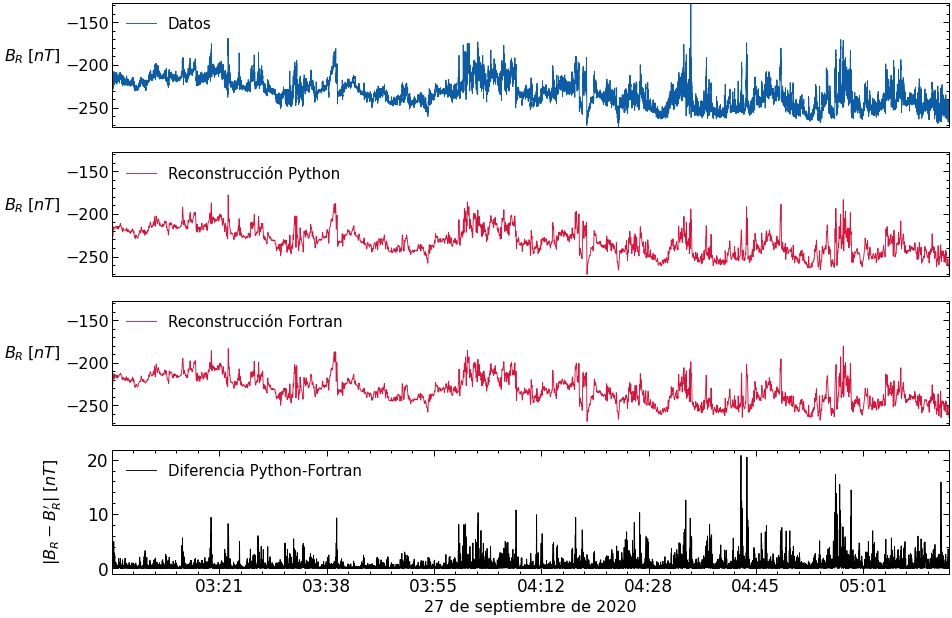
\includegraphics[scale=0.43]{Imagenes/reconstruction_PSP.png}
    \caption{Reconstrucciones de la serie temporal $B_{R}$ de PSP a partir de sus IMFs. De arriba hacia abajo: señal, reconstrucción de Python con $80\%$ IMFs, reconstrucción de Fortran con $75\%$ IMFs, valor absoluto de la diferencia entre las reconstrucciones.}
    \label{fig:reconstruction_PSP}
\end{figure}

\begin{figure}[H]
    \centering
    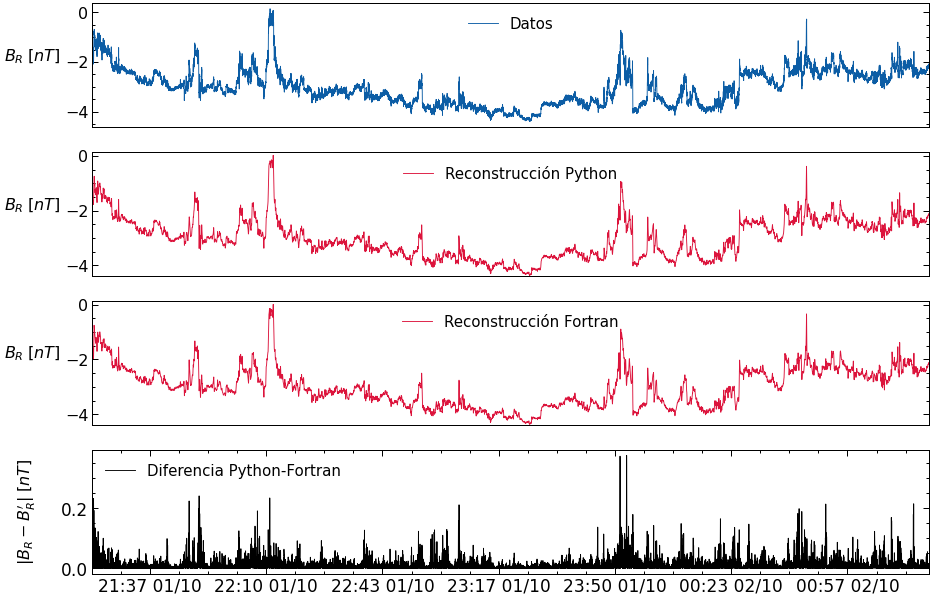
\includegraphics[scale=0.43]{Imagenes/reconstruction_SolO.png}
    \caption{Similar a la figura \ref{fig:reconstruction_PSP} pero para los datos de SolO.}
    \label{fig:reconstruction_SolO}
\end{figure}

Las reconstrucciones de la serie temporal con todas sus IMFs mostraron una diferencia del orden de la precisión de los datos ($\sim 10^{-13}-10^{-14}$). Más aún, los datos originales y las diferentes reconstrucciones con todas las IMFs también dieron estos resultados. Por tanto, a pesar de que las diferentes implementaciones generan un número diferente de IMFs, los resultados entre sí son comparables. Esto valida nuestra implementación realizada en Fortran. 

En la figura \ref{fig:reconstruction_SolO} se muestran las reconstrucciones parciales de la serie temporal $B_{R}$ de SolO, a partir de las IMFs de menor frecuencia en la figura \ref{fig:emdSolO}. Ambas reconstrucciones utilizan $8$ IMFs. En este caso las reconstrucciones parciales se parecen mucho más a la serie temporal original que en los datos de PSP. 

\begin{figure}[H]
\centering
\subfigure{\includegraphics[scale=0.36]{imfs_SolO_fortran.png}\label{emdSolO:1}}
\subfigure{\includegraphics[scale=0.36]{imfs_SolO_python.png}\label{emdSolO:2}}
\caption{Similar a la figura \ref{fig:emdPSP} pero para los datos de SolO. Izquierda: Fortran, 11 IMFs; derecha: Python, 10 IMFs.}
\label{fig:emdSolO}
\end{figure}

\subsection{Correlaciones a baja frecuencia entre ventanas de tiempo de las series temporales}

\noindent En esta sección presentamos los resultados de nuestro análisis exploratorio. Estos resultados se obtuvieron a través de la implementación del método EMD de Python. Resultados similares se obtuvieron con las IMFs calculadas en nuestra implementación de Fortran. 

Debido al poco tiempo disponible para realizar este trabajo, solamente se pudo analizar una de las componentes del campo magnético, y se decidió que fuera la componente radial. Esta componente es predominante en las series temporales estudiadas (en promedio, $B$ y $B_{R}$ son casi paralelas) \cite{telloni_evolution_2021}. Más aún, no todas las componentes son afectadas de la misma manera por la turbulencia del viento solar, pues esta es anisotrópica \cite{duan_anisotropy_2021}. A medida que crece la distancia respecto del Sol, la anisotropía de las fluctuaciones también crece \cite{bruno_effects_1999}, en relación con la evolución de la turbulencia. Sin embargo, las fluctuaciones son mayores en la dirección perpendicular al campo medio que en la dirección paralela \cite{belcher_large-amplitude_1971}. En este caso la componente radial es la menos afectada por la turbulencia. Las razones anteriores hacen que el seguimiento de la componente radial del campo magnético sea más interesante en un primer acercamiento exploratorio, y que el análisis del resto de las componentes vaya más allá del alcance de este estudio.    

El barrido se realizó con ventanas de 10 a 88 minutos en pasos de 2 minutos. El tiempo de desplazamiento ($d$) también fue de 2 minutos. Por otro lado, en el barrido de las IMFs se sumaron hasta 10 componentes de las series temporales, respecto de la implementación del EMD de Python. Esto hizo que el número de operaciones necesarias para el cálculo de las correlaciones en los barridos propuestos fuera superior a $10^4$. Estas operaciones consumieron mucho tiempo computacional y por esta razón se omitieron las ventanas de mayor duración (que son las que tardan más tiempo en computar).    

En la figura \ref{fig3} se muestran los máximos de correlación obtenidos en los barridos de las ventanas de tiempo y las IMFs. Resalta que la tendencia de estos máximos, respecto de todas las ventanas, no varía mucho cuando se consideran más de 5 IMFs en la reconstrucción de las series temporales. Considerar menos de 4 IMFs genera correlaciones altas como consecuencia de una reducción significativa de la información de las series, por la acción del filtrado. 

\begin{figure}
    \centering
    \includegraphics[scale=0.55]{barrido_imfs.png}
    \caption{Máximos de correlación en el barrido sobre la duración de las ventanas de tiempo y el número de IMFs. Entre líneas puntadas se separan tres rangos de ventanas de tiempo para los que se observaron diferentes patrones de correlación relevantes en las series temporales de $B_{R}$.}
    \label{fig3}
\end{figure}

\begin{figure}
\centering
\subfigure[$\Delta t = 20$ minutos]{\includegraphics[scale=0.42]{mapa_corr/fig-20&2.png}\label{fig6: 1}}
\subfigure[$\Delta t = 28$ minutos]{\includegraphics[scale=0.42]{mapa_corr/fig-28&2.png}\label{fig6: 2}}
\subfigure[$\Delta t = 36$ minutos]{\includegraphics[scale=0.42]{mapa_corr/fig-36&2.png}\label{fig6: 3}}
\subfigure[$\Delta t = 44$ minutos]{\includegraphics[scale=0.42]{mapa_corr/fig-44&2.png}\label{fig6: 4}}
\subfigure[$\Delta t = 52$ minutos]{\includegraphics[scale=0.42]{mapa_corr/fig-52&2.png}\label{fig6: 5}}
\subfigure[$\Delta t = 80$ minutos]{\includegraphics[scale=0.42]{mapa_corr/fig-80&2.png}\label{fig6: 6}}
\caption{Mapas de correlaciones para algunas ventanas de tiempo en las series temporales de $B_{R}$ de PSP y SolO. Las correlaciones se calcularon entre datos reconstruidos con 4 IMFs de baja frecuencia. De arriba hacia abajo y de izquierda a derecha: ventanas de tiempo de 20, 28, 36, 44, 52 y 80 minutos.}
\label{fig6}
\end{figure}

Si los valores máximos de una matriz de correlaciones (como la figura \ref{scan}), calculados para una amplitud de ventana, se visualizan en un mapa de calor entonces se pueden observar patrones característicos como los de la figura \ref{fig6}. Estos \textit{mapas de correlaciones} se obtuvieron de las reconstrucciones con las 4 IMFs de menor frecuencia, pues lo observado en la figura \ref{fig3} sugiere que 4 es el número mínimo de IMFs que permiten obtener un buen filtrado de las series y mantener la tendencia de los máximos de correlación, respecto de las series no filtradas. Los valores de la figura \ref{fig3} se corresponden con los máximos de cada uno de los mapas de correlaciones, es decir, aquellos obtenidos en los barridos de las ventanas de tiempo y las IMFs.

Los patrones observados indican que las series temporales contienen varios intervalos de tiempo, de diferente duración, donde su correlación es máxima. En particular, las regiones de mayor correlación para las ventanas entre 22 y 54 minutos fueron relevantes. En este rango de ventanas, los máximos de correlación de la figura \ref{fig3} tienen gradientes pronunciados, disminuyendo rápidamente hasta los 36 minutos y con un pico en los 44 minutos, para después continuar con la tendencia decreciente. Asimismo, podemos notar que alrededor de las ventanas de 22 y 54 minutos existen cambios relativamente grandes en la correlación, para las reconstrucciones con más de 4 IMFs. Además, los intervalos de tiempo que les corresponden a este rango de ventanas se solapan con aquellos que contienen al mismo plasma espacial en las series temporales del campo magnético.   

Las otras ventanas no mostraron mapas de correlaciones con regiones bien definidas y con una diferencia notoria respecto del resto del mapa. Esto lo podemos observar en los paneles \ref{fig6: 1} y \ref{fig6: 6}. Además, para cada IMF, las ventanas menores a 22 minutos presentan máximos de correlación muy altos y casi no varían mucho entre sí, posiblemente debido a que se consideran pocos datos para hacer las cuentas. En el caso de ventanas de más de 54 minutos puede que la semejanza entre las series temporales disminuya y por eso menos intervalos de tiempo muestran alta correlación. En las ventanas de más de 80 minutos se observa un incremento en el máximo de la correlación, aunque los mapas de correlación muestran una única región poco localizada, es decir, valores altos muy dispersos. Esto simplemente reduce los posibles intervalos de tiempo que se pueden relacionar con la presencia del mismo plasma.    

Las tres bandas de ventanas sombreadas de la figura \ref{fig3} se relacionan con las regiones de correlación relevantes de la figura \ref{fig6}. Sólo las bandas donde la correlación disminuye muestran dos regiones localizadas. La banda central es algo así como una transición entre las regiones de las otras bandas. A pesar de la alta correlación de las regiones observadas, no es la alta correlación lo relevante en este estudio. Los cambios significativos en la correlación a medida que se añaden más IMFs son de interés. Quizá las ventanas donde existe un gran salto en la correlación, ya sea para un número determinado de IMFs o al variar las IMFs, podrían ser físicamente significativas. Por ejemplo, en la figura \ref{fig3}, las reconstrucciones con 4 IMFs destacan estos saltos para las ventanas de $22$ y $54$ minutos.

Los expertos suelen utilizan series temporales cuya duración es superior a los $60$ minutos para sus estudios \cite{telloni_evolution_2021}. La razón de esto es que para tiempos de menor duración la turbulencia tiende a destruir las estructuras de menor tamaño o provoca que la correlación entre estas (estructuras) disminuya mucho durante la expansión del viento solar \cite{bruno_turbulence_2016}. Sin embargo, los tiempos encontrados ($\sim 22 - 54$ minutos), con este análisis de carácter puramente exploratorio, podrían tener alguna relevancia física, más allá de la relación con los intervalos de tiempo que contienen al mismo plasma espacial, y por tanto se deberían estudiar más detenidamente para descubrir su importancia.

\begin{figure}
    \centering
    \includegraphics[scale=0.52]{barrido_ventanas_celdas.png}
    \caption{Máximos de correlación respecto del número de IMFs de menor frecuencia que reconstruyen las ventanas de tiempo de las series temporales de $B_{R}$. Las ventanas de 44 y 54 minutos se indican con marcadores diferentes como ejemplo de la tendencia.}
    \label{fig4}
\end{figure}    

En las figuras \ref{fig4} y \ref{fig5} se muestran resultados similares a lo observado en la figura \ref{fig3}. El máximo de correlación no varía mucho para las reconstrucciones con más de 5 IMFs. Además, en la figura \ref{fig4} se observa que el máximo de correlación en cada uno de los mapas se incrementa al reducir el número de IMFs de las señales y que disminuye al considerar ventanas más grandes. Por otro lado, la figura \ref{fig5} indica que los intervalos de tiempo más correlacionados, con 10 IMFs (cuando no se han filtrado las altas frecuencias), no siempre incrementan su correlación al reducir el número de IMFs en la reconstrucción de las señales.          

La reconstrucción de las series temporales de $B_{R}$ con $5$ IMFs mostró una frecuencia característica (frecuencia en el valor máximo del espectro de potencias de Fourier justo antes del comportamiento de ley de potencia en la curva $log-log$; el lector puede dirigirse a las referencias para más detalles, en particular \cite{carbone_arbitrary-order_2018}) de $9\times 10^{-3} Hz$ para PSP y  $1.66\times 10^{-3} Hz$ para SolO. Estos valores son cercanos a la frecuencia característica de la quinta IMF de menor frecuencia, $1\times 10^{-2} Hz$ para PSP y $4.16\times 10^{-3} Hz$ para SolO, lo cual es esperado por la acción del filtro. Estos valores de frecuencia podrían sugerir una escala característica para identificar cuándo las partes no turbulentas de dos series temporales del campo magnético del viento solar están altamente correlacionadas y quizá verificar si pertenecen al mismo plasma. Sin embargo, mayores detalles sobre las implicaciones físicas no son del todo claros y se necesita un mayor estudio.

\begin{figure}
    \centering
    \includegraphics[scale=0.52]{barrido_ventanas_celda_serie.png}
    \caption{Similar a \ref{fig4} pero para las particiones de mayor correlación que se obtienen con la serie temporal completa, es decir, las particiones son fijas en el barrido.}
    \label{fig5}
\end{figure}

\begin{figure}
    \centering
    \includegraphics[scale=0.45]{reconstruccion_54min_0&30.png}
    \caption{Reconstrucción de las series temporales de $B_{R}$ con las 4 IMFs de menor frecuencia en una ventana de 54 minutos. Arriba: datos de PSP en el intervalo de tiempo 03:15-04:09 UT el 27 de septiembre de 2020; abajo: datos de SolO en el intervalo de tiempo 22:20-23:14 UT el 01 de octubre de 2020.}
    \label{fig7}
\end{figure}

\begin{figure}
    \centering
    \includegraphics[scale=0.45]{reconstruccion_54min_23&18.png}
    \caption{Similar a \ref{fig7}. Arriba: datos de PSP en el intervalo de tiempo 04:01-04:55 UT el 27 de septiembre de 2020; abajo: datos de SolO en el intervalo de tiempo 21:56-22:50 UT el 01 de octubre de 2020.}
    \label{fig8}
\end{figure}

En las figuras \ref{fig7} y \ref{fig8} se presenta el caso particular de la reconstrucción de las series temporales (de PSP y SolO) con 4 IMFs de baja frecuencia, para dos ventanas de tiempo de 54 minutos. Se observa que las reconstrucciones se ajustan suavemente al comportamiento de los datos. El valor máximo de la función cross-correlation entre las señales reconstruidas es de $0.705$ para la figura \ref{fig7} y $0.656$ para la figura \ref{fig8}. Los intervalos de tiempo están relacionados con cada una de las regiones relevantes en los mapas de correlación, teniendo los pares de ventanas más correlacionados para 54 minutos. Estos intervalos son entre las horas 03:15 - 04:09 UT del 27 de septiembre de 2020 en PSP y 22:20 - 23:14 UT del 1 de octubre de 2020 en SolO.  Por otro lado, los intervalos de tiempo de las otras reconstrucciones son entre las horas 04:01 - 04:55 UT en PSP y 21:56 - 22:50 UT en SolO, en los días respectivos.  

Las series temporales analizadas en este trabajo se corresponden con los intervalos de tiempo ampliados que se estudiaron en la investigación que se toma de referencia \cite{telloni_evolution_2021}. En otras palabras, no se asegura que toda la duración de las señales pertenece al mismo plasma espacial, sino solamente una parte. Los intervalos de tiempo encontrados, en las regiones de alta correlación, están contenidos o se solapan con aquellos hallados en el estudio anterior, indicando nuevamente que los intervalos reportados son los que contienen la información del mismo plasma espacial.

\section{Conclusiones y recomendaciones}

\noindent Nuestra implementación del método EMD en Fortran produjo, en promedio, un mayor número de IMFs respecto de las implementaciones profesionales en Matlab y Python. Esta diferencia se debe al grado de optimización de las implementaciones. Sin embargo, los resultados fueron comparables dado que la reconstrucción de las series temporales fue similar. Esto permitió validar la implementación hecha en Fortran. 

El cálculo de las correlaciones propuestas se limitó a la componente radial del campo magnético. En el barrido sobre el número de IMFs se estimó que alrededor de 5 IMFs, con la implementación de Python, permiten reconstruir las series de forma adecuada, realizar un buen filtrado de las altas frecuencias y mantener la tendencia de los máximos de correlación para las distintas amplitudes de ventana, con respecto a las series no filtradas.     

Por otro lado, el barrido de las ventanas de tiempo mostró que ventanas entre 22 y 54 minutos presentan una alta correlación (\ref{fig6}) y que sus valores máximos tienen gradientes pronunciados (\ref{fig3}), que los diferencian de ventanas menores a 22 minutos o mayores a 54 minutos. Esto sugiere que las amplitudes de ventana entre 22 y 54 minutos podrían ser físicamente significativas. Sin embargo, este estudio, que tiene un carácter puramente exploratorio, sólo permitió identificar estas amplitudes, pero no se pudo concluir nada sobre sus implicaciones físicas pues los detalles no son del todo claros. Por último, los intervalos de tiempo, asociados a estas amplitudes de ventana, se solapan con aquellos reportados en el estudio anterior \cite{telloni_evolution_2021} sobre los datos analizados en este trabajo, es decir, se relacionan con la información del mismo plasma a distintas distancias.

Finalmente, se recomienda estudiar las propiedades físicas, de la parte no turbulenta de las series temporales, de las ventanas de tiempo entre 22 y 54 minutos para su determinar su relevancia y sus posibles implicaciones físicas. También, un trabajo que siguiera la línea iniciada en este estudio debería investigar las frecuencias características de las reconstrucciones de las series con 5 IMFs y buscar si existe algún significado físico. De igual manera, se debe continuar explorando sobre las otras componentes del campo magnético y revisar el número de IMFs para obtener un buen filtro de las altas frecuencias. 
